% !TeX root = ../../thesis.tex

Table \ref{tab:allvsall} shows the aggregated metrics for AUROC, AUPRC, RMSE and MAE for distributed, centralised and local models predicting capabilities on each silo. The data refers to the mean of the metric values for all columns tested as targets for all methods and all silos. We also calculated the 95\% confidence interval for each model (local and distributed per silo) in order to assess how well the distributed model would work as opposed to the local one per silo. We also calculated the p Value for the means of the distributed vs centralised and distributed vs local.
%TC:ignore
%\setlength{\tabcolsep}{7pt} % Default value: 6pt
%\renewcommand{\arraystretch}{1.3} % Default value: 1

\begin{table}[h!] 
 \setlength{\tabcolsep}{7pt} % Default value: 6pt 
 \renewcommand{\arraystretch}{1.3} % Default value: 1
  \captionsetup{justification=centering} 
\centering
\caption[Metrics for centralised model, distributed model and local model]{Comparison of the distributed model with the centralised model and with the local model (Mean for all model and all columns). 2-sample T-test for the means was used as hypothesis test. Bold for \textit{P} value below 0.05. AUPRC and AUROC for categorical target variable and RMSE and MAE for continuous target variable.}

\label{tab:allvsall}
\begin{tabular}{llcccc}
\toprule
 &  & M & SD & 95\% CI & \textit{P}  \\
\midrule
\multirow{3}{*}{AUPRC}
 & distributed & 0.691 & 0.216 & (0.686, 0.696) & - \\
  & centralised & 0.706 & 0.225 & (0.701, 0.711) & \bfseries 1.10e-17 \\
 & local & 0.659 & 0.220 & (0.654, 0.665) & \bfseries 4.71e-05 \\
 \hline

\multirow{3}{*}{AUROC} 
 & distributed & 0.723 & 0.182 & (0.718, 0.727) & - \\
 & centralised & 0.729 & 0.180 & (0.725, 0.734) & \bfseries 2.98e-26 \\
 & local & 0.692 & 0.164 & (0.688, 0.695) & \bfseries 2.48e-02 \\

\hline

\multirow{3}{*}{MAE} 
 & distributed & 2.370 & 1.608 & (2.315, 2.425) & - \\
 & centralised & 2.365 & 1.923 & (2.298, 2.431) & \bfseries 2.23e-04 \\
 & local & 2.527 & 1.799 & (2.465, 2.589) & 9.01e-01 \\

\hline

\multirow{3}{*}{RMSE} 
 & distributed & 21.171 & 46.078 & (19.584, 22.757) & - \\
 & centralised & 19.839 & 28.645 & (18.853, 20.826) & \bfseries 2.92e-02 \\
 & local & 23.771 & 49.776 & (22.057, 25.485) & 1.63e-01 \\
\hline
\end{tabular}
\end{table}





%TC:endignore

Figure \ref{fig:heatmap-cat} shows the AUROC of each algorithm and silo on the Y axis and target variable and type of model on the X. The color bar refers to the value of the AUROC. Blue being lower values and red bigger values. The same type of graph was created for regression, where the Figure \ref{fig:heatmpa-int} shows the MAE for each silo and algorithm and target variable and type of model. 


%TC:ignore

\begin{figure}[h!]
\centering
\captionsetup{justification=centering}

\caption[Heatmap of classification algorithm and silo vs Target variable and model type.]{Heatmap of classification algorithm and silo vs Target variable and model type. Value is the AUROC mean of all 10 experiments. Y axis is the algorithm and silo. X axis is Target variable and Method. AA - Position Admission; ANP - Position on Delivery; AGESTA - Nr of Pregnancies; APARA - Nr of born babies; GS - Blood Group; GR - Robson Group; TG -Pregnancy Type; TP - Delivery Type; TPEE - Spontaneous Delivery; TPNP - Actual Type of Delivery; V - Followed physician; VCS - Followed physician primary care; VNH - Followed physician hospital delivery;}\label{fig:heatmap-cat} 
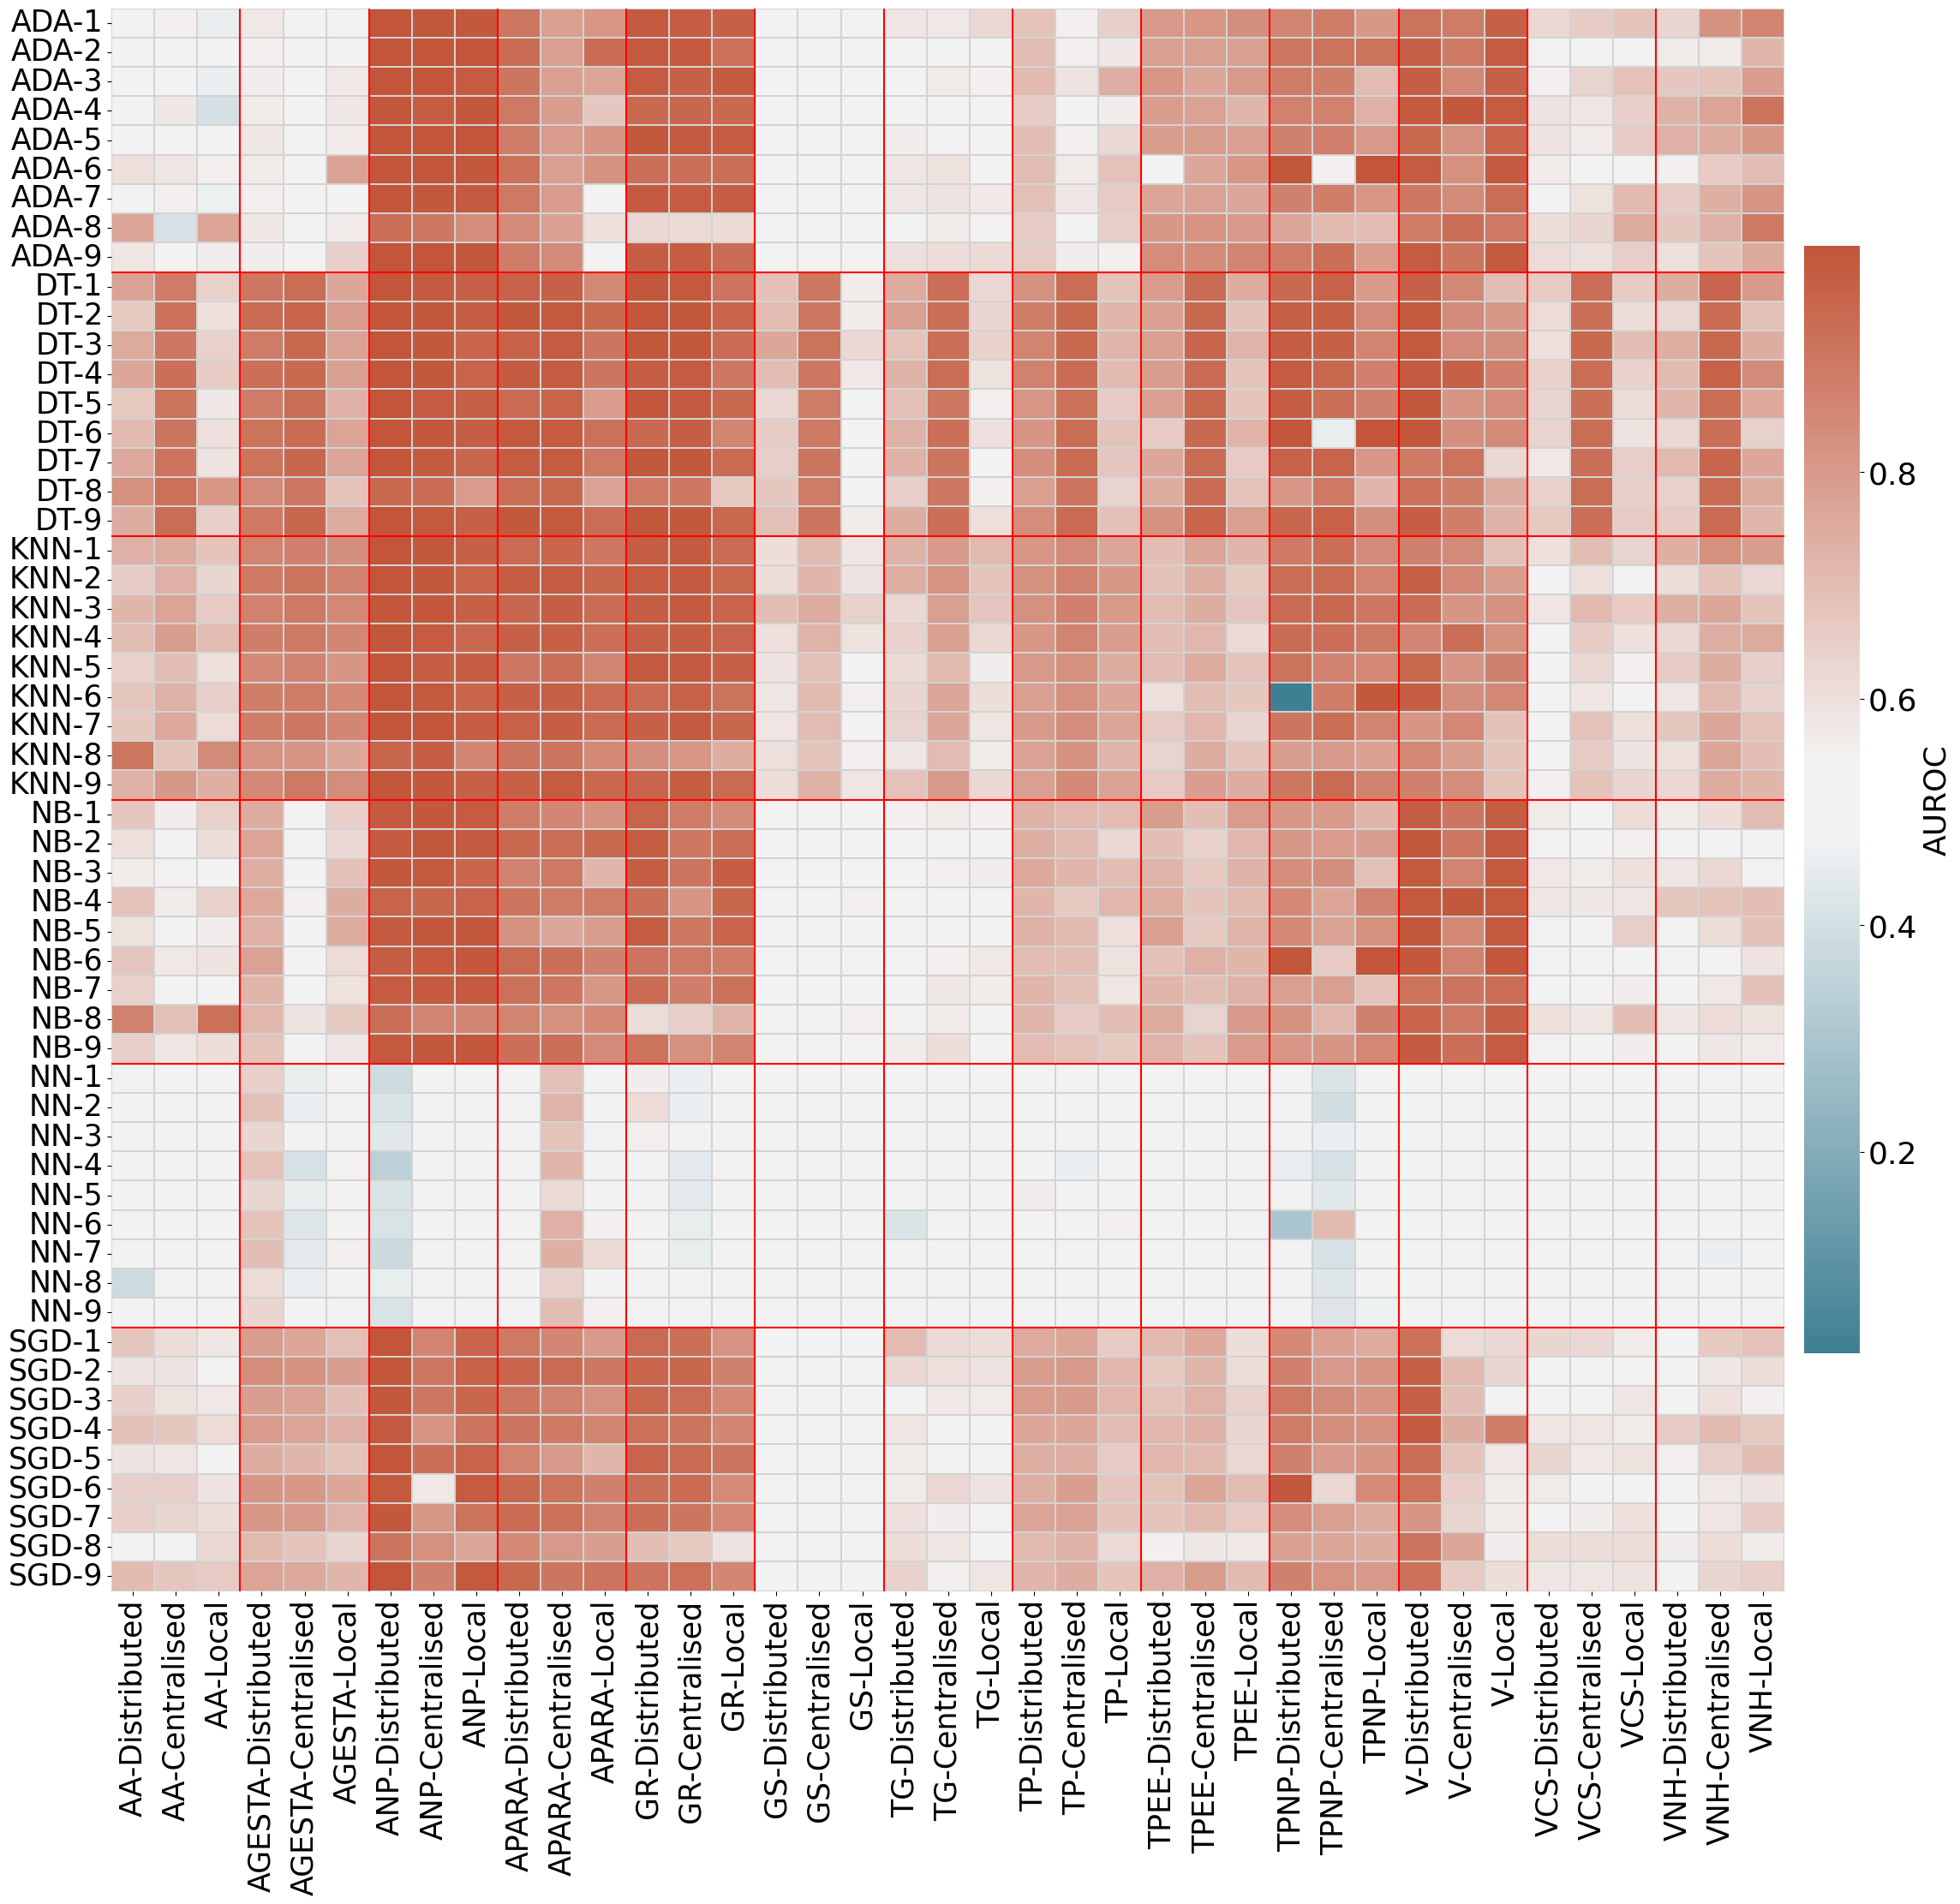
\includegraphics[scale=0.22]{figures/heatmap-class.png}
\end{figure}
%TC:endignore
%TC:ignore

\begin{figure}[htbp]
\centering
\captionsetup{justification=centering}

\caption[Heatmap of regression algorithm and silo vs Target variable and model type.]{Heatmap of regression algorithm and silo vs Target variable and model type. Value is the MAE mean of all 10 experiments. The y axis is the algorithm and silo. X axis is Target variable and Method. IA - Mother Age; IGA - Weeks on Admission; IMC - BMI; NRCPN - Nr of consultations; PI - Weight start of pregnancy; SGP - Weeks on Delivery;}\label{fig:heatmpa-int} 
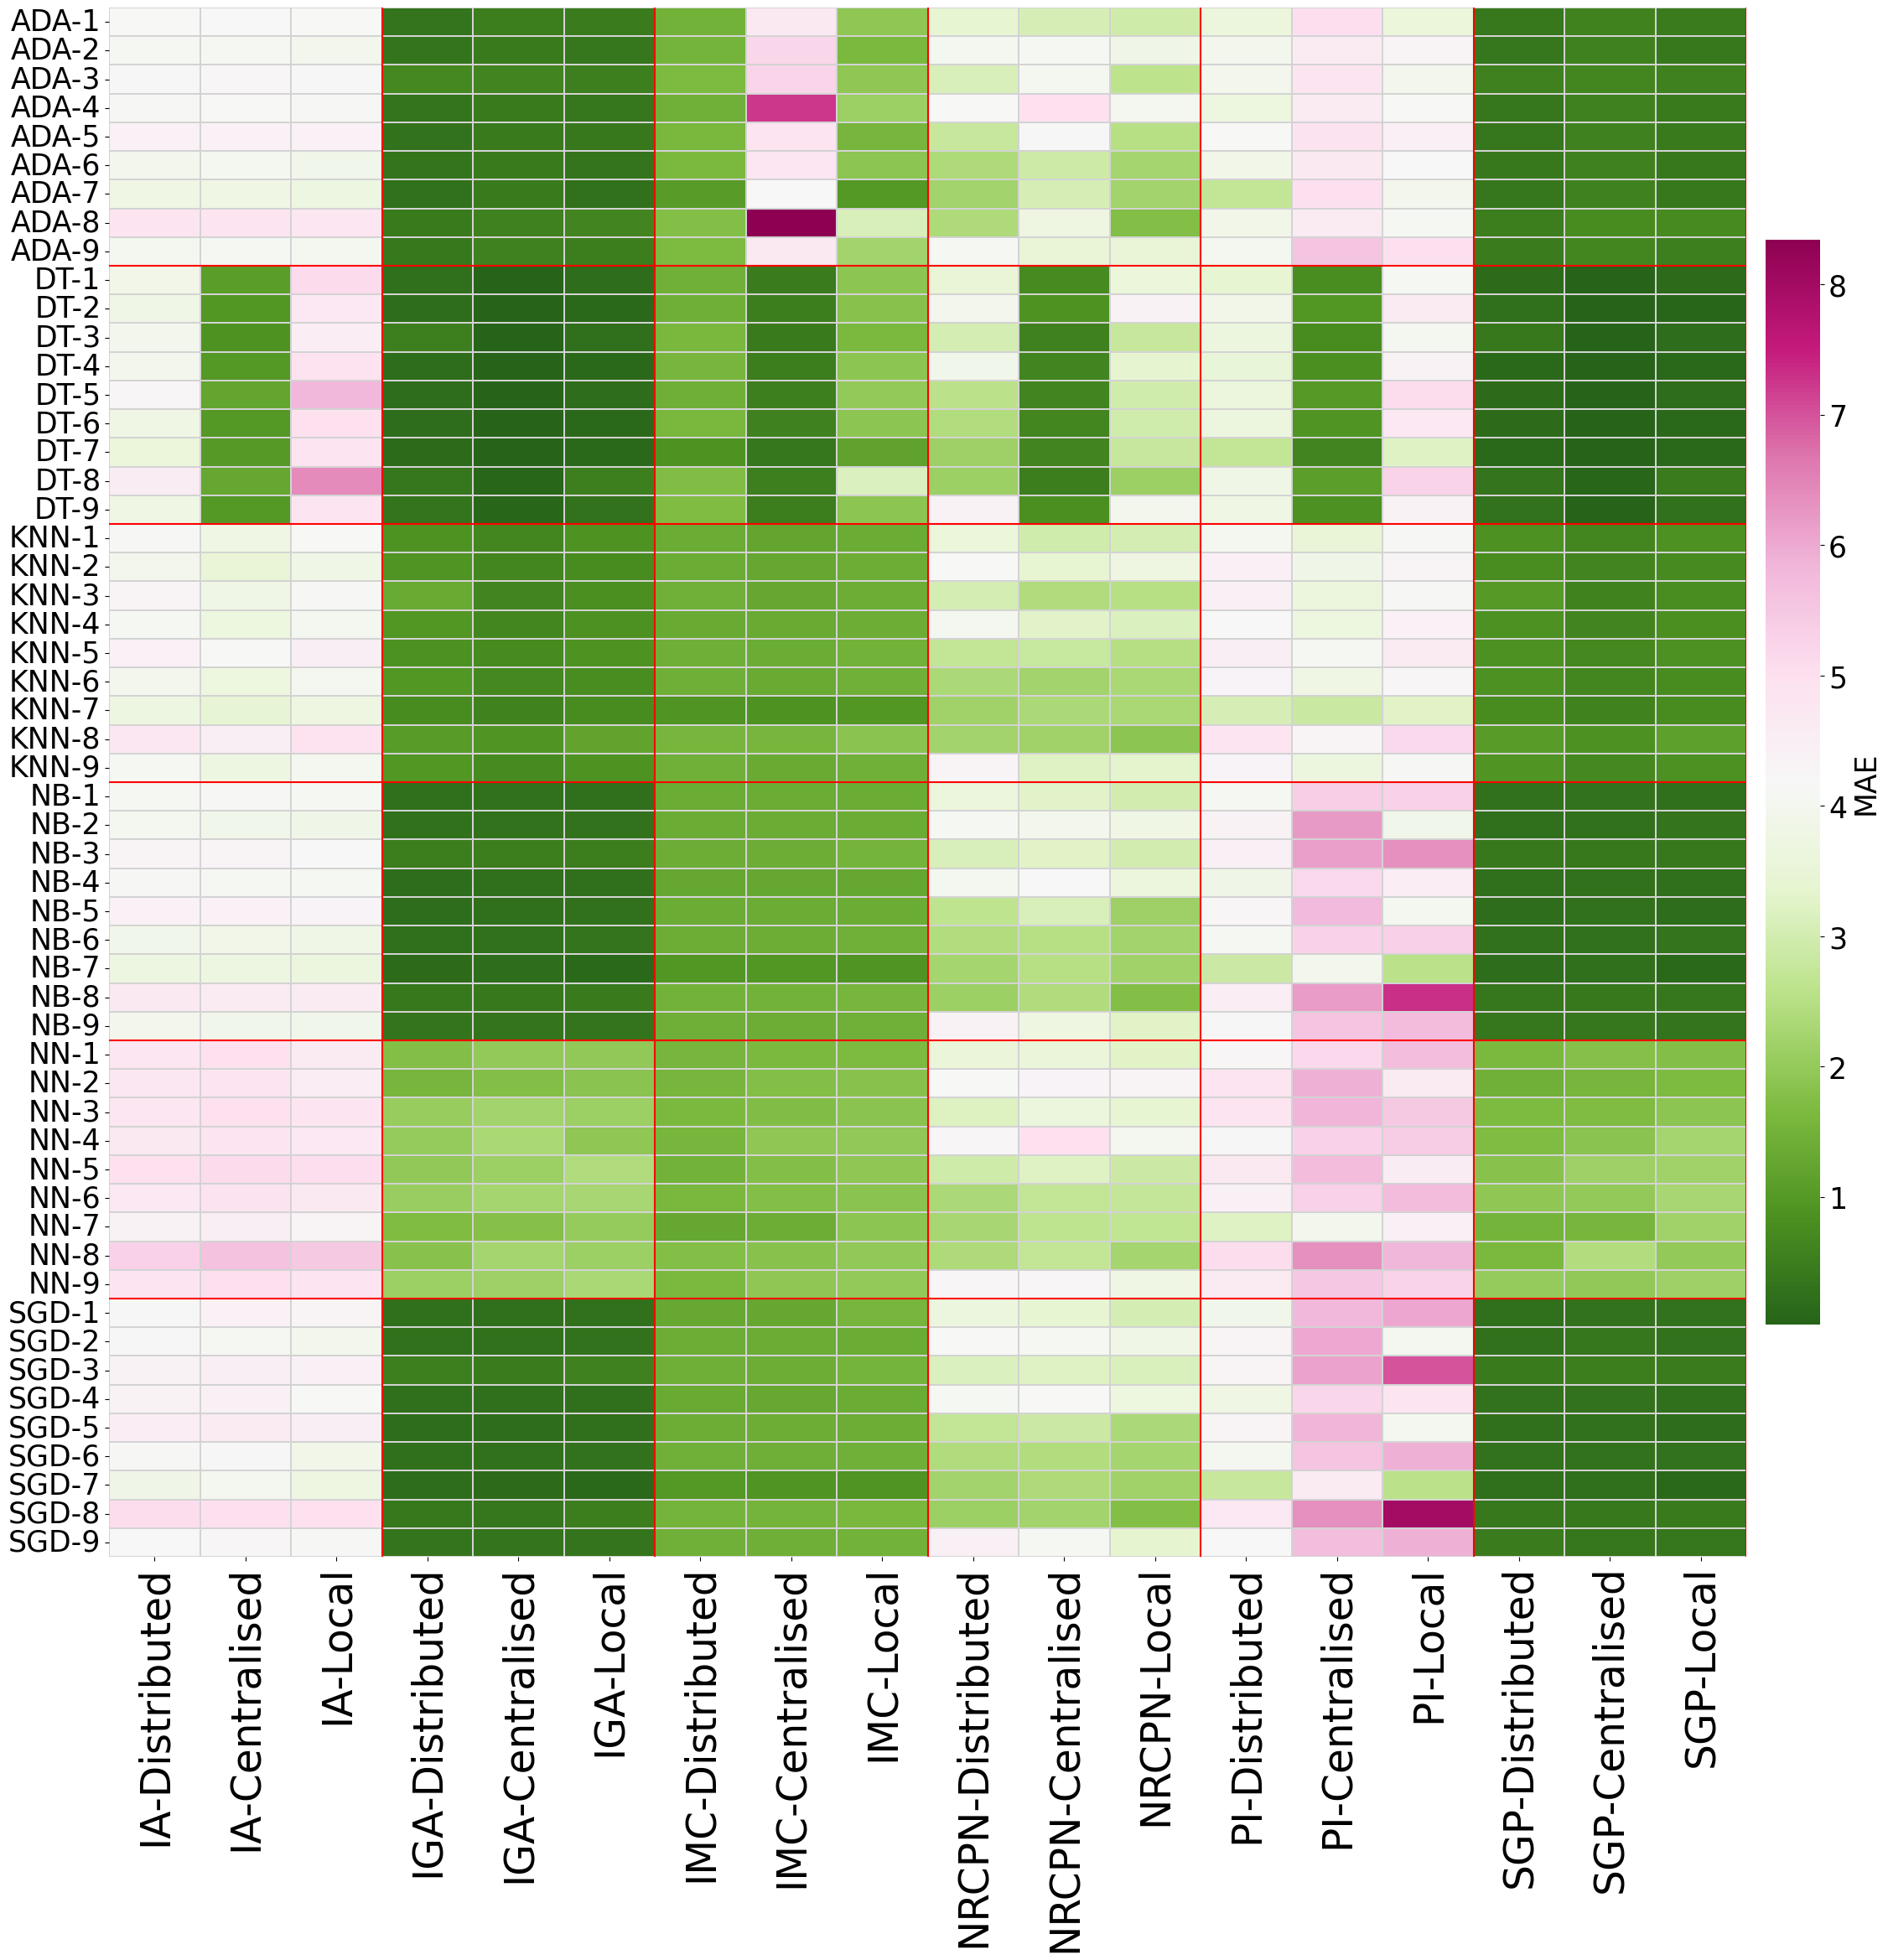
\includegraphics[scale=0.22]{figures/heatmap-reg.png}
\end{figure}
%TC:endignore

{\small
\definecolor{Gray}{gray}{0.85} 
 \begin{table}[h] 
 \setlength{\tabcolsep}{6pt} % Default value: 6pt 
 \renewcommand{\arraystretch}{1.1} % Default value: 1
  \captionsetup{justification=centering} 
\centering
\caption[Model comparison: Distributed versus centralised and local for every test]{Model comparison: Distributed versus centralised and local for every test. Each cell is the total of distributed model when compared with centralised model (row) and local model (column) across different silos and outcome variable. ($>$ for better, = for non significance and $<$ for worse). The first example is 72 which means that 72 iterations of the distributed SGD was better than the centralised and local. SGD: Stochastic Gradient Descent, NN: Neural Network, KNN: K-Nearest Neighbors, ADA: AdaBoost, NB: Naive Bayes, DT: Decision Tree. Comparison was done with 2-sample T-test with a $\alpha$ of 0.05. (\% in parentheses)}
\label{tab:hyp}
\begin{tabular}{llrrrr}
\toprule


 &  & Distributed $>$ Local & Distributed = Local & Distributed $<$ Local & \textbf{Row Total} \\


\hline \multirow{3}{*}{SGD} &Distributed $>$ Centralised  & 72 (7.0) & 14 (1.4) & 9 (0.8) & \textbf{95 (9.3)} \\
 & Distributed =  Centralised& 14 (1.4) & 17 (1.7) & 6 (0.6) & \textbf{37 (3.6) } \\
 & Distributed $<$ Centralised  & 11 (1.1) & 11 (1.1) & 17 (1.7) & \textbf{39 (3.8)} \\
% \hline
% \multicolumn{2}{c|}{SGD Total} & 97 (9.4)&42 (4.1) &32 (18.7)& \textbf{171}  \\
\hline \multirow{3}{*}{NN} & Distributed $>$ Centralised & 44 (4.3) & 44 (4.3) & 7 (0.7) & \textbf{95 (9.3)} \\
 & Distributed =  Centralised& 2 (0.2) & 33 (3.2) & 2 (0.2) & \textbf{37 (3.6)} \\
 & Distributed $<$ Centralised & 0 (0) & 17 (1.7) & 22 (2.1) & \textbf{39 (3.8)} \\
% \hline

% \multicolumn{2}{c|}{NN Total} & 46&94 &31 & \textbf{171}  \\

\hline \multirow{3}{*}{KNN} & Distributed $>$ Centralised & 16 (1.6) & 0 (0) & 1 (0.1) & \textbf{17 (1.7)} \\
 & Distributed =  Centralised & 10 (1) & 2 (0.2) & 1 (0.1) & \textbf{13 (1.3)} \\
 & Distributed $<$ Centralised & 72 (7)  & 28 (2.7) & 41 (4) & \textbf{141 (13.7)} \\
% \hline

% \multicolumn{2}{c|}{KNN Total} & 97&30 &43 & \textbf{171}  \\

\hline \multirow{3}{*}{ADA} & Distributed $>$ Centralised & 64 (6.2) & 25 (2.4) & 22 (2.1) & \textbf{111 (10.8)} \\
 & Distributed =  Centralised& 5 (0.5) & 12 (1.2) & 10 (1) & \textbf{27(2.6)} \\
 & Distributed $<$ Centralised & 10 (1) & 6 (0.6) & 17 (1.7) & \textbf{33 (3.2)} \\
% \hline

% \multicolumn{2}{c|}{ADA Total} & 79&43 &49 & \textbf{171}  \\

\hline \multirow{3}{*}{NB} & Distributed $>$ Centralised & 51 (5) & 19 (1.9) & 34 (3.3) & \textbf{104 (10.1) } \\
 &  Distributed =  Centralised & 5 (0.5) & 19 (1.9) & 12 (1.2) & \textbf{36 (3.5)} \\
 & Distributed $<$ Centralised  & 3 (0.3) & 4 (0.4) & 24 (2.3) & \textbf{31 (3)} \\
% \hline

% \multicolumn{2}{c|}{NB Total} & 59&42 &70 & \textbf{171}  \\

\hline \multirow{3}{*}{ DT} & Distributed $>$ Centralised & 27 (2.6) & 0 (0) & 1 (0.1) & \textbf{28 (2.7)} \\
 & Distributed = Centralised & 8 (0.8) & 0 (0) & 0 (0)& \textbf{8 (0.8)} \\
 & Distributed $<$ Centralised & 97 (9.5) & 12 (1.2) & 26 (2.5) & \textbf{135 (13.2)} \\
% \hline

% \multicolumn{2}{c|}{DT Total} & 132&12 &27 & \textbf{171}  \\
 
 \hline
  \textbf{Total} &  & \textbf{511 (49.8)} & \textbf{263 (25.6)} & \textbf{252 (24.6)} & \textbf{1026 (100)}\\
 \bottomrule
\end{tabular}
\end{table}
}















